%Author - Akshay Vijayvergia
% $DA-IICT ID$ 201401061.


\documentclass[11pt]{article}

\oddsidemargin  -0.0in
\textwidth      6.5in
\headheight     0.0in
\topmargin      -0.25in
\textheight     9.0in
\parindent      0.0in
\parskip        0.05in

\usepackage{epsfig}
\usepackage{listings}

%used to include animation
\usepackage{animate}
\usepackage{animfp}

\begin{document}

% ---------------------------------------------------------------------------

\begin{center}
{\large SC462 Elements of Synthetic Biology: Life 2.0} \\
Prof. Manish K Gupta \\
DA-IICT\\
\hspace{0.25in} \\
{\Large\bf Cello: genetic circuit design automation} \\
Akshay Vijayvergia
\end{center}

% ---------------------------------------------------------------------------

\section*{ Cello}
\subsection*{Abstract}
DNA is the single most important part of all the organisms present on the planet. It consists of the genetic instructions used in the functioning, growth and development of all known living organisms. Due to this, to study biological architecture, we need to perform computations in living cells by DNA-encoded circuits which indeed process sensory information and control all the biological functions. But due to the various complexions like time and design, the computations become close to impossible. Thus to tackle this problem, we study Cello, which serves as a design environment where the user gives a verilog code as input that is automatically transformed into a DNA sequence providing a genetic circuit design. 

%%%%%%%%%%%%%%%%%%%%%
\subsection*{Introduction}
Cello is a web based open source tool that is used to build genetic circuit diagrams. Its input consists of a Verilog script. This script is then parsed into a truth table which is further synthesised to generate a genetic circuit diagram with the genetically available gate types in the library. For simulating the circuit, a predicted score guides a breadth-first search, or a Monte Carlo simulated annealing search. Among all the predicted scores, the one with the highest score is selected. The one which is selected could then be implemented using the various genetic layouts. For finalising among one or more DNA sequences for the designated circuit, the Eugene language is used which further processes upon the rule based combinatorial design.


%%%%%%%%%%%%%%%%%%%%%
\subsection*{Verilog Specification}
When opening the website http://www.cellocad.org/verilog.html, we are greeted with a text editor which enables us to input the Verilog script. Cello accepts three forms of verilog scripts namely case statements, assign statements and structural statements. The verilog programs usually start with module keyword, followed by the name taking a list of output and input wire names as its arguments. We now focus on all the three specified verilog types.

Case
This style is usually preferred when we directly want to specify the truth table for our circuit.

\begin{figure}[ht!]
\centering
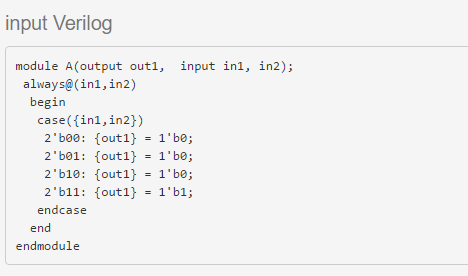
\includegraphics[width=4cm,height=5cm,keepaspectratio]{Screenshot_1.png}
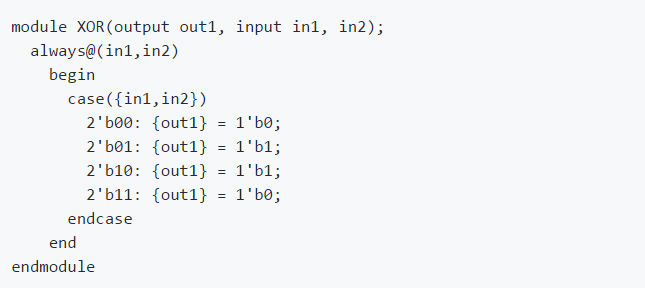
\includegraphics[width=11cm,height=12cm,keepaspectratio]{Screenshot_2.png}
\label{Case exmaple}
\end{figure}





\end{document}